\chapter{Auswertung}
\markboth{Auswertung}{}
\label{ch:Auswertung}

Nach der Optimierung der Struktur der Transaktionserfassung \bzgl der einzelnen Komponenten durch Auslagern von einzelner Modulen, der Umkehrung der Abhängigkeiten zwischen Komponenten und Auflösung von Komponenten in bestehende und neue Komponenten, haben sich bestimmte Eigenschaften verbessert. Darunter fällt, dass der Abhängigkeitsbaum nicht mehr gegen das \ac{SDP} verstößt. Die Komponenten, die Schnittstellen zu anderen Systemen, die die Benutzeroberfläche, Datenbank oder einem SMTP Server darstellen, sind auf eine höhere Schicht verschoben worden. Somit verweist eine höher gelegene Schicht nur noch auf eine niedrigere Schicht (\refAbb{fig:schichten}). 

\begin{figure}
  \centering
  \includegraphics[width=0.7\textwidth]{res/schichten.jpg}
   \caption{Schichtmodell mit Verortung der Komponenten nach der Restrukturierung der Transaktionserfassung von WBS Alarm.}
   \label{fig:schichten}
\end{figure}

In \refTabns{tab:comp_transaktion_vergleich} wird die Entwicklung der einzelnen Kennzahlen verglichen. Die Komponenten \code{core}, \code{http} und \code{entity} sind dabei gleich geblieben, \bzw haben sich nicht signifikant geändert. Durch die Abhängigkeitsumkehr von \code{repository} zu \code{action} wurde eine neue Verbindung zu \code{entity} aufgebaut, weshalb sich dort $I_{entity}$ von 0,56 auf 0,55 verringert hat.

Merklicher haben sich die Werte der anderen Komponenten geändert. Durch Einführung einer neuen Schnittstelle und dem Herauslösen einer Klasse hat sich $A_{action}$ um 0,14 erhöht. Durch die stärkere Verwendung von außen hat sich allerdings gleichzeitig $I_{action}$ um 0,04 verringert. Insgesamt hat sich durch die stärkere Abstraktion $D_{action}$ von 0,21 auf 0,31 erhöht.

Durch die Verschiebung der Komponente \code{repository} auf die äußerste Schicht konnte $D_{repository}$ von 0,60 auf 0,00 verbessert werden. In \refTabns{tab:comp_transaktion_vergleich} wurden mit Stern markierte Werte nach der Argumentation \bzgl der Schnittstellen zur Datenbank mittels \textit{Spring Boot Data} aus Kapitel~\ref{ch:Vorgehensweise} angepasst. 

Die Kompente \code{service} konnte komplett aufgelöst werden, was zur Einhaltung des \ac{SDP} beigetragen hat. Das Modul für die Berechtigungsprüfung mittels JPQL wurde mit in die \code{TransaktionsDaoImpl} aufgenommen (\refLst{lst:n_TransaktionDaoImpl}, Zeile 44--72). Das zweite Modul wurde in die neue Komponente \code{mail} ausgelagert (\refLst{lst:n_MailServiceImpl}).

Die Streudiagramme in \refAbbns{fig:diagramm_ist} und \refAbbns{fig:diagramm_refac} zeigen die Verteilung der Komponenten vor und nach der Anpassung. Es wird deutlich, dass sich weniger Komponenten abseits der Hauptreihe befinden.

\begin{table}[]
\centering
\caption{Änderung der Abstraktheit $A$, Instabilität $I$ und Abstand zur Hauptreihe $D$ vor und nach der Restrukturierung im Vergleich.}
\label{tab:comp_transaktion_vergleich}
\begin{tabular}{@{}l|rr|rr|rr@{}}
\toprule
\multirow{2}{*}{Komponente} & \multicolumn{2}{c|}{$A$} & \multicolumn{2}{c|}{$I$} & \multicolumn{2}{c}{$D$} \\
                  & alt    & neu    & alt  & neu  & alt    & neu    \\ \midrule
\code{action}     &   0,25 &   0,39 & 0,96 & 0,93 &   0,21 &   0,31 \\
\code{core}       &   0,67 &   0,67 & 0,00 & 0,00 &   0,33 &   0,33 \\
\code{entity}     &   0,00 &   0,00 & 0,56 & 0,55 &   0,44 &   0,45 \\
\code{http}       &   0,00 &   0,00 & 1,00 & 1,00 &   0,00 &   0,00 \\
\code{repository} & * 0,00 & * 0,00 & 0,40 & 1,00 & * 0,60 & * 0,00 \\
\code{service}    &   0,00 &   -    & 0,58 & -    &   0,42 & -      \\
\code{mail}       &   -    &   0,00 & -    & 1,00 & -      &   0,00 \\
\bottomrule
\end{tabular}
\end{table}


\begin{figure}
  \centering
  \includegraphics[width=0.55\textwidth]{res/diagramm_ist.jpg}
   \caption{Streudiagramm der Komponenten über Abstraktheit $A$ und Instabilität $I$ vom Ausgangszustand der Transaktionserfassung in WBS Alarm.}
   \label{fig:diagramm_ist}
\end{figure}


\begin{figure}
  \centering
  \includegraphics[width=0.55\textwidth]{res/diagramm_refac.jpg}
   \caption{Streudiagramm der Komponenten über Abstraktheit $A$ und Instabilität $I$ nach Restrukturierung und Anwendung der Design"= und Komponentenprinzipien auf die Transaktionserfassung in WBS Alarm.}
   \label{fig:diagramm_refac}
\end{figure}

Insgesamt ist die Vorgehensweise zielführend. Durch die Analyse der Komponenten und der Visualisierung der Abhängigkeiten kann ermittelt werden, an welchen Stellen gegen Komponentenprinzipien verstoßen wird. Durch die Designprinzipien konnte eine Lösung modelliert werden. Dabei musste festgelegt werden, welche Aufgabe eine Komponente erfüllen soll und in welcher Schicht sie sich, angelehnt am Schichtmodell (\refAbb{fig:clean_architecture}), befinden sollte. \ac{DIP} hat sich als nützlichstes Designprinzip herausgestellt, da durch die Abhängigkeitsregel falsch verknüpfte Komponenten leicht umstrukturiert werden konnten.

In dieser Arbeit wurde nur die Transaktionserfassung von WBS Alarm berücksichtigt, wodurch sich neue Aufgabenstellungen im Gesamtsystem ergeben haben, welche die Umkehr von \code{repository} zu \code{action} mit sich gebracht haben. In \code{action} haben  die in dieser Arbeit nicht betrachteten Usecases die Beziehung zu \code{repository} nicht geändert. Dadurch wurde hier eine bidirektionale Verbindung aufgebaut. Durch die in dieser Arbeit gesammelten Erfahrungen mit der Transaktionserfassung können aber die gleichen Prinzipien angewendet werden, um diesen Missstand zu beheben.
